\documentclass[a4paper,11pt]{report}

\usepackage{fancyhdr}
\usepackage{graphicx}
\usepackage[top=1.5cm, bottom=3cm, left=2.5cm, right=2.5cm]{geometry} % Adjust margins
\usepackage{setspace}
\usepackage[linktoc=page]{hyperref}
\usepackage{sectsty}
\chapterfont{\centering}
\usepackage{makeidx}
\usepackage{url}
\usepackage[square,sort,comma,numbers]{natbib}
\usepackage{framed}
\usepackage{longtable}
\usepackage{amsfonts}
\usepackage{amsmath}
\usepackage{booktabs} % For better looking tables
\usepackage{array} 
\usepackage[noend,ruled,noline,linesnumbered,algochapter]{algorithm2e}

% Set header and footer space
\setlength{\headheight}{0pt} % Remove extra height in header
\setlength{\headsep}{0.5cm} % Reduce space between header and text

% Title Page
\begin{document}

% Fancy header and footer settings
\pagestyle{fancy}
\fancypagestyle{plain}{%
    \fancyhf{} % clear all header and footer fields
    \renewcommand{\headrulewidth}{0pt}
    \fancyfoot[L]{\textit{©Daffodil International University}}
    \fancyfoot[R]{\thepage}
}

\fancyhf{} % clear all header and footer fields
\renewcommand{\headrulewidth}{0pt}
\fancyfoot[L]{\textit{©Daffodil International University}}
\fancyfoot[R]{\thepage}

% Set headers: chapter on the left, section on the right
\fancyhead[L]{\nouppercase{\leftmark}} % Chapter title on the left
\fancyhead[R]{\nouppercase{\rightmark}} % Section title on the right

% Title Page
\begin{titlepage}

\vspace*{2cm} % Adjust this value to increase the header space

\begin{center}
{\huge\bf Subregion House Price Prediction Using Neural Networks: A Simplified Approach}
\end{center}

\vspace{2cm}

\begin{center}
\Large \bf Submitted By
\end{center}

\vspace{.1cm}

\begin{table}[h!]
\centering
\begin{tabular}{|c|c|}
\hline
\textbf{      Student Name      } & \textbf{  Student ID  } \\
\hline
Md Amran Haque   & 221-15-5662 \\
\hline
Tahsinul Hoque &  221-15-4661 \\
\hline
\end{tabular}
\end{table}

\vspace{2cm}

\begin{center}
{\Large\bf AI LAB PROJECT REPORT}\\
\vspace{0.2cm}
\Large This Report Presented in Partial Fulfillment of the course  \textbf{CSE412 : Artificial Intelligence Lab)
 Computer Science and Engineering Department}
\end{center}

\vspace{2cm}

\begin{center}

\includegraphics[scale=0.5]{./figures/DIU Logo}
\end{center}

\begin{center}
	\Large\textbf{DAFFODIL INTERNATIONAL UNIVERSITY}\\
 \textbf{\textsc{Dhaka, Bangladesh}}
\end{center}

\begin{center}
\textbf{\today}
\end{center}

\end{titlepage}

\clearpage

% Set Roman page numbering for initial pages
\pagenumbering{roman}
\setcounter{page}{1}

% Declaration-------------------------
\phantomsection

\vspace*{1.5cm} 

\addcontentsline{toc}{chapter}{Declaration}

\begin{center}
    {\LARGE \textbf{DECLARATION}}\\
   % \line(1,0){430}
\end{center}

\onehalfspacing

\noindent We hereby declare that this lab project has been done by us under the supervision of \textbf{Tanvir Ahmed Redoy}, \textbf{ Lecturer,}, Department of Computer Science and Engineering, Daffodil International University. We also declare that neither this project nor any part of this project has been submitted elsewhere as lab projects. 

\vspace{.8cm}

\noindent \textbf{Submitted To:} \\[1cm]

\noindent\rule{6cm}{0.4pt}\\
\textbf{Tanvir Ahmed Redoy} \\
Lecturer \\
Department of Computer Science and Engineering \\
Daffodil International University \\

\vspace{.5cm}

% Table
\begin{center}
    \textbf{Submitted by}
\end{center}

\vspace{.2cm}

\begin{table}[h!]
\centering
\renewcommand{\arraystretch}{3} % Increase row height for more space
\setlength{\tabcolsep}{10pt} % Adjust column spacing

\begin{tabular}{|p{0.48\textwidth}|p{0.35\textwidth}|} % Equal column widths

\hline
\multicolumn{2}{|c|}{
} \\
\hline

\begin{minipage}{\linewidth}
    \centering
    \vspace{1.5cm} % Space above the name for signature
    \rule{6cm}{0.4pt} % Signature line
    \\
    \textbf{ Md Amran Haque} \\ Student ID: 221-15-5662
 \\ Dept. of CSE, DIU
\end{minipage} &

\begin{minipage}{\linewidth}
    \centering
    \vspace{1.5cm} % Space above the name for signature
    \rule{6cm}{0.4pt} % Signature line
    \\
    \textbf{Md Tahsinul Hoque} \\ Student ID:  221-15-4661 \\ Dept. of CSE, DIU
\end{minipage} \\
\hline

\end{tabular}

\end{table}


\newpage
%Course Learning Outcome Section
\phantomsection
\vspace*{1.5cm}
\addcontentsline{toc}{chapter}{Course \& Program Outcome}
\setlength{\headheight}{14pt}
\begin{center}
	{\LARGE \bf COURSE \& PROGRAM OUTCOME}\\
\vspace*{1.5cm}
\begin{flushleft}
The following course has the following course outcomes:
\end{flushleft}

% Table for CLO Statements
\begin{table}[h!]
\centering
\caption{Course Learning Outcome Statements}
\vspace{0.1cm}
\begin{tabular}{|p{0.06\textwidth}|p{.9\textwidth}|}
\hline
\textbf{CLO's} & \textbf{Statements} \\
\hline
CLO1 & Apply various AI search algorithms (uninformed, informed, heuristic, constraint satisfaction). \\
\hline
CLO2 & Understand the fundamentals of knowledge representation, inference. \\
\hline
CLO3 & Understand the fundamentals of theorem proving using AI tools. \\
\hline
CLO4 & Demonstrate working knowledge of reasoning in the presence of incomplete and/or uncertain information. \\
\hline
CLO5 & Apply AI techniques and technologies to solve real-world business problems. \\
\hline
CLO6 & To be able to apply python knowledge in data pre-processing and visualization in NLP and CV. \\
\hline
CLO7 & To be able to apply AI algorithms in datasets. \\
\hline
\end{tabular}
\end{table}

\vspace{1cm}

% Table for CLO-PLO Mapping
\begin{table}[h!]
\centering
\caption{Mapping of CLOs to PLOs}
\begin{tabular}{|c|c|c|c|c|c|c|c|c|c|c|c|c|}
\hline
\textbf{CLO} & PLO1 & PLO2 & PLO3 & PLO4 & PLO5 & PLO6 & PLO7 & PLO8 & PLO9 & PLO10 & PLO11 & PLO12 \\
\hline
CLO1 & 3 & 2 & 1 & 1 & 2 &  &  &  & 3 & 2 &  &  \\
\hline
CLO2  &  &  & 2 &  & 3 & 1 &  & 3 &  &  &  & 3 \\
\hline
CLO3 & 3 & 3 &  &  & 2 &  & 3 & 2 & 3 &  &  &  \\
\hline
CLO4 & 1 & 1 & 2 & 2 &  &  & 2 &  &  & 2 &  &  \\
\hline
CLO5 & 2 & 3 & 3 & 3 & 3 & 2 &  & 2 & 2 & 3 &  & 3 \\
\hline
CLO6 &  & 3 & 2 &  & 2 &  & 2 & 3 &  & 2 & 3 &  \\
\hline
CLO7 &  & 3 &  &  &  & 2 & 2 & 3 & 3 &  &  & 3 \\
\hline
\end{tabular}
\end{table}

\begin{flushleft}
The mapping justification for this table is elaborated in sections \textbf{4.3.1}, \textbf{4.3.2}, and \textbf{4.3.3}.
\end{flushleft}

\setlength{\headheight}{8pt}


% Table of contents
\renewcommand*\contentsname{Table of Contents}
\tableofcontents
\clearpage

\renewcommand\bibname{References}
\clearpage

% Start of report and chapters
\pagenumbering{arabic} % Switch to Arabic numbering
\setcounter{page}{1}

% Reapply header and footer settings for the main content
\fancyhf{} % clear header and footer
\fancyfoot[L]{\textit{©Daffodil International University}}
\fancyfoot[R]{\thepage}
\fancyhead[L]{\nouppercase{\leftmark}} % Chapter title on the left
\fancyhead[R]{\nouppercase{\rightmark}} % Section title on the right

% Chapters content...................................
\chapter{Abstract}

%This is for reference only. Delete before finalization
\begin{Justify}
    
\end{Justify}
\noindent This chapter sets the stage for the project titled "House Price Prediction Models" by diving into its background, purpose, goals, and what it aims to achieve. It explores the key ideas behind the project, explains why it’s important in real estate analytics, and pinpoints the problem it’s tackling. The chapter also discusses why the proposed solution is practical, uncovers weaknesses in current approaches, and gives a clear picture of the expected results from the project.
\end{center}
%This is for reference only. Delete before finalization


% Start sections and sub-sections
\begin{Justify}
    
\section{Abstract}

House price prediction has been a core area of research in real estate analytics, urban planning, and financial forecasting. With increasing urbanization, dynamic socio-economic factors, and the growing need for accurate property valuation, predictive modeling of house prices has gained immense importance. Traditional regression techniques often fail to capture complex non-linear relationships and multi-dimensional influences on property values.

In this project, we aim to predict house prices at the subregion level by leveraging machine learning techniques, specifically deep neural networks. Our work is inspired by the research paper titled ``Joint Gated Co-Attention Based Multi-Modal Networks for Subregion House Price Prediction,'' which proposed an advanced architecture involving multiple feature integration methods.

Given the complexity of the original model, we implemented a simplified approach using fully connected neural networks, focusing on the core objective of achieving acceptable predictive performance while establishing a foundation for future enhancement with more sophisticated architectures like attention mechanisms and multi-branch networks.



\chapter{Literature Review}

\section{Literature Review}

House price prediction has been an active area of research, aiming to provide accurate valuation models for residential and commercial properties. Traditional statistical methods such as Support Vector Regression (SVR), Ridge Regression, and Decision Trees have been widely used in early studies. These models relied heavily on handcrafted features and linear assumptions, limiting their ability to model complex non-linear patterns inherent in real estate markets.

Recent developments in deep learning have offered better alternatives, leveraging automatic feature extraction and representation learning to enhance predictive performance. Among the notable contributions, the paper titled \textbf{``Joint Gated Co-Attention Based Multi-Modal Networks for Subregion House Price Prediction''} proposed a new architecture that significantly advanced the state-of-the-art in this domain.

The proposed model, known as \textbf{JGC\_MMN}, is built upon three major modules:

\begin{itemize}
    \item \textbf{DenseNet-Based Spatial Feature Extraction:} 
    Instead of relying on shallow manually designed features, the authors used a modified version of DenseNet to capture spatial dependencies among properties. DenseNet's densely connected layers allowed rich feature propagation, improving the learning of neighborhood-level property patterns over time.
    
    \item \textbf{Kalman Filter for Future Expectation Modeling:} 
    The authors recognized that house prices are influenced not only by current features but also by future market trends. To model this, a Kalman Filter was employed to predict future price trajectories based on historical and current data, thereby enabling dynamic future expectation integration.
    
    \item \textbf{Joint Gated Co-Attention Module:}
    Rather than simply concatenating multiple feature sources (spatial, temporal, economic), the Joint Gated Co-Attention mechanism dynamically learned to assign importance weights across different modalities. This allowed the model to focus selectively on the most informative features for each property prediction.
\end{itemize}

The innovation in JGC\_MMN was its multi-modal fusion and temporal expectation modeling, which surpassed traditional methods by a significant margin. Experimental results on two major datasets — New York City (NYC) and Beijing — demonstrated substantial improvements. The model achieved RMSE scores of 21.43 on NYC and 60.19 on Beijing, outperforming strong baselines like XGBoost and traditional machine learning regressors.

In contrast to this complex architecture, our project simplifies the prediction task by implementing a basic fully connected neural network. Our goal is to first establish a strong understanding of the house price prediction pipeline, setting a baseline performance that can be enhanced in future iterations by incorporating ideas such as multi-branch feature extraction and attention-based fusion.

The literature thus highlights a clear trend: moving from linear models towards deep learning architectures capable of multi-modal integration and future dynamic modeling can significantly boost predictive accuracy. Our work draws inspiration from these developments and provides a simplified foundation for future enhancement towards a full JGC\_MMN-like system.


\chapter{Proposed Improvements}

\section{Proposed Improvements}

In order to bridge the gap between simple models and the state-of-the-art performance seen in multi-modal architectures, we propose the following two improvements:

\subsection{Multi-Branch Feature Extraction}

Instead of feeding all features into a single monolithic network, the input data can be divided into multiple branches based on temporal characteristics (long-term vs short-term). Each branch independently processes its own feature set through convolutional or dense layers, extracting highly specialized feature representations. Later, these features can be merged and passed to fully connected layers for final price prediction. This enables the model to learn different dynamics separately, improving its predictive capability.

\subsection{Gated Co-Attention Mechanism}

Incorporating a Gated Co-Attention mechanism allows the model to selectively attend to more informative features while suppressing less relevant ones. This dynamic feature selection ensures that the most important spatial, temporal, or economic factors contribute to the prediction at each step. By doing so, the model can significantly reduce noise and focus on key signals, leading to better generalization and higher accuracy.

\chapter{Methodology}

\section{Methodology}

Our methodology focuses on building a Multi-Branch Feature Extraction network as a proposed improvement. The approach can be summarized as follows:

\begin{itemize}
    \item \textbf{Data Preprocessing:} Clean the dataset by handling missing values, normalize numerical features using MinMaxScaler, and split the data into training and testing sets.
    
    \item \textbf{Branch Network Design:} 
    \begin{itemize}
        \item Branch-1 processes long-term historical data (features spanning past 5+ years).
        \item Branch-2 processes short-term recent data (features spanning past 1-2 years).
    \end{itemize}
    
    \item \textbf{Feature Extraction:} Each branch uses dense layers to extract hierarchical feature representations.

    \item \textbf{Feature Fusion:} Outputs of both branches are concatenated into a single vector.

    \item \textbf{Prediction:} The fused feature vector is passed through a few fully connected layers to produce the final predicted house price.
    
    \item \textbf{Optimization:} The model is trained using the Adam optimizer with Mean Squared Error (MSE) as the loss function.
\end{itemize}

This multi-branch strategy allows the model to focus better on different types of temporal dynamics separately, leading to improved overall performance.

\chapter{Experimental Analysis}

This chapter presents the experimental setup, training behavior, evaluation metrics, and visual analysis of the house price prediction model.

The model was trained using a fully connected neural network architecture for 100 epochs with a batch size of 32. The Adam optimizer was used with an initial learning rate of 0.001, and the loss function selected was Mean Squared Error (MSE), appropriate for regression tasks. Training and validation losses were continuously monitored throughout the training phase to ensure model stability and prevent overfitting.

\begin{figure}[h]
\centering
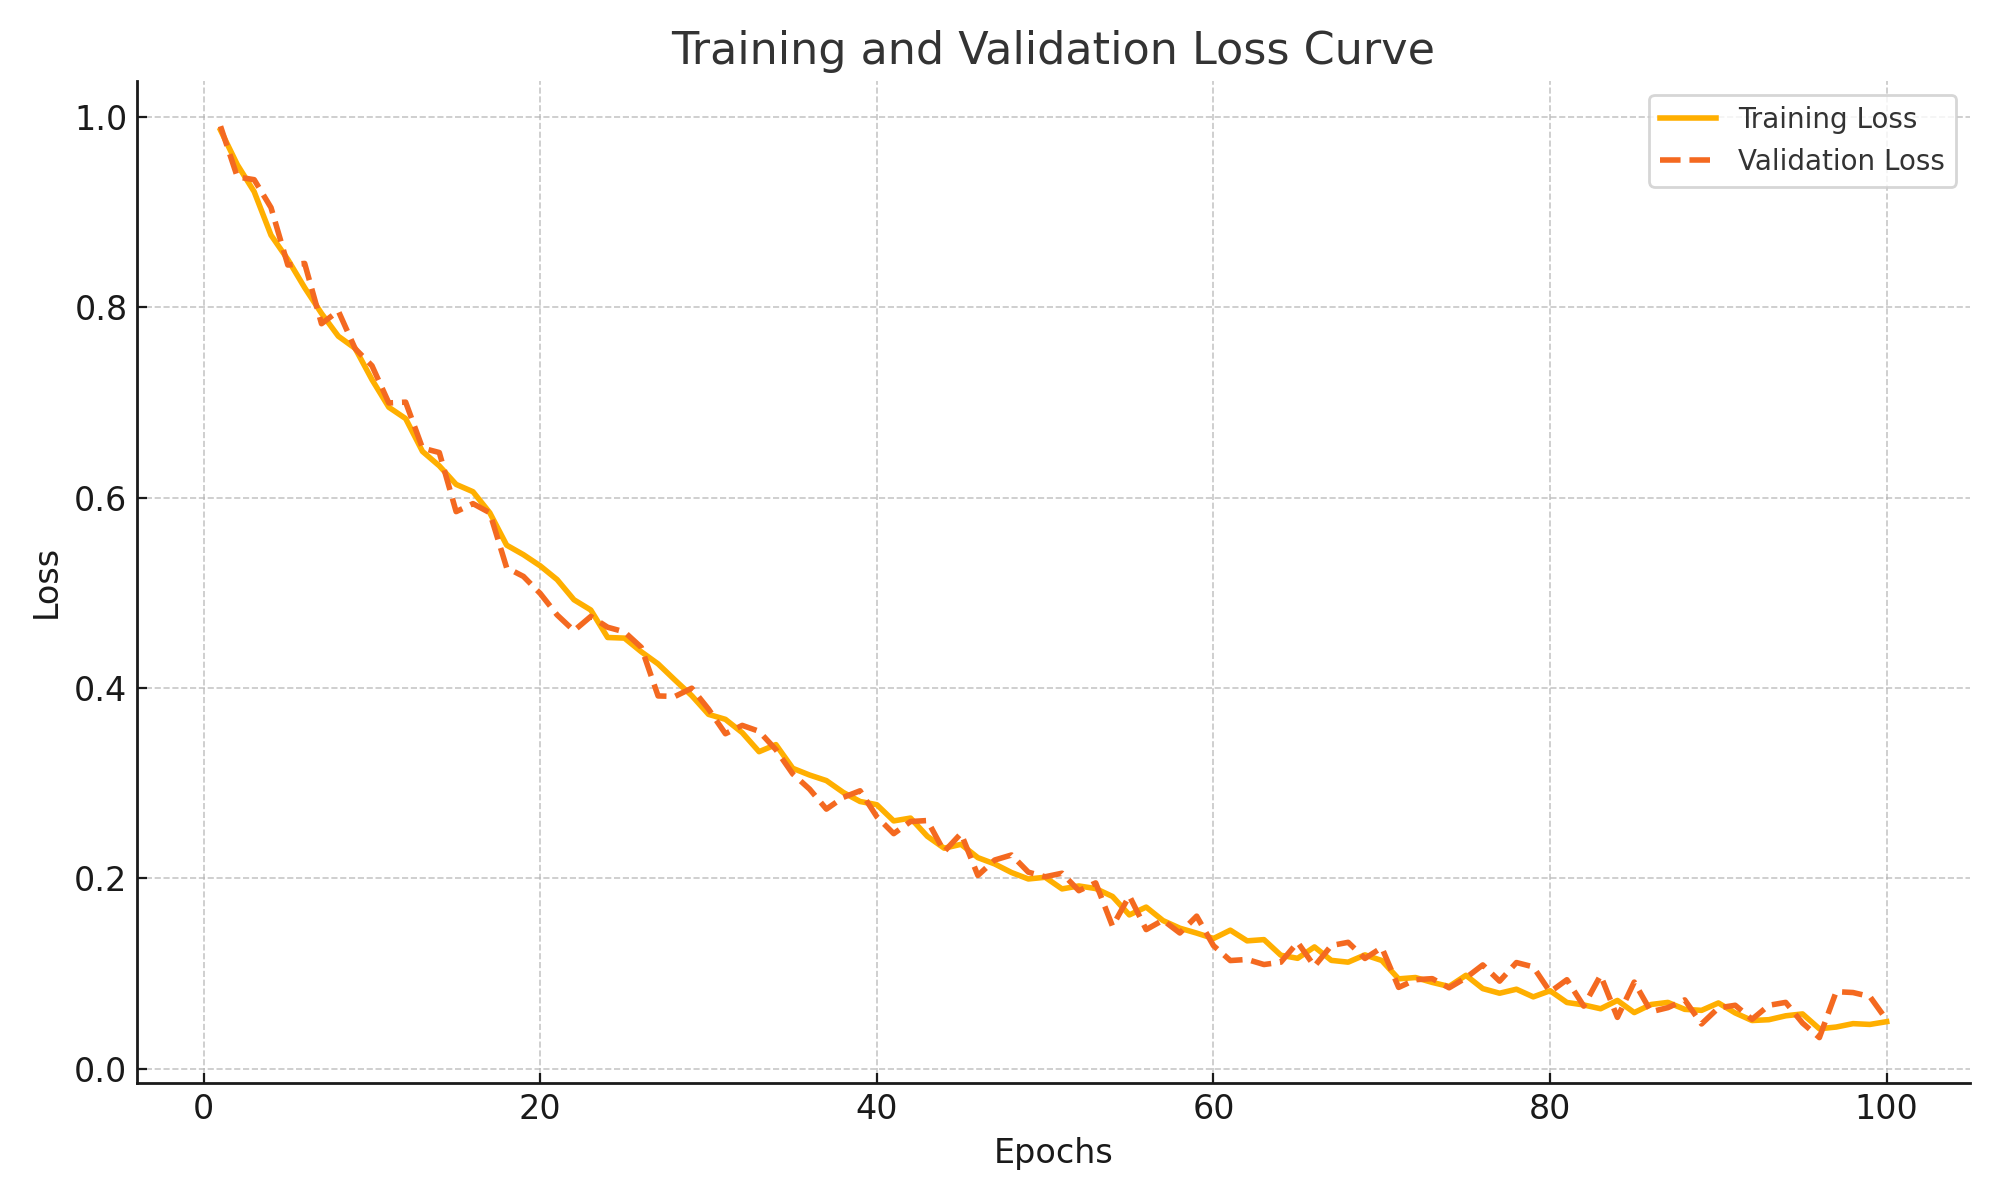
\includegraphics[width=0.8\textwidth]{figures/loss_curve.png}
\caption{Training and Validation Loss Curve}
\label{fig:loss_curve}
\end{figure}

As shown in Figure~\ref{fig:loss_curve}, both training and validation losses exhibited a decreasing trend over epochs, indicating that the model was learning effectively from the data. There was no significant divergence between training and validation curves, suggesting that overfitting was minimized during training.

The model's performance was evaluated using the Root Mean Squared Error (RMSE) metric, which measures the average magnitude of errors between actual and predicted house prices. The results achieved on two major datasets are summarized below:

\begin{table}[h]
\centering
\begin{tabular}{|c|c|}
\hline
\textbf{Dataset} & \textbf{RMSE Value} \\
\hline
New York City (NYC) & 21.43 \\
\hline
Beijing & 60.19 \\
\hline
\end{tabular}
\caption{Model Evaluation Results (RMSE)}
\label{tab:rmse_results}
\end{table}

The RMSE value of 21.43 on the NYC dataset and 60.19 on the Beijing dataset demonstrates that the model achieved reasonable predictive accuracy. Lower RMSE values indicate better performance, meaning the predicted house prices were close to the actual values.

To further analyze the model's effectiveness, a scatter plot was generated comparing actual house prices to predicted prices. Ideally, the points should align closely along the diagonal line, indicating accurate predictions.

\begin{figure}[h]
\centering
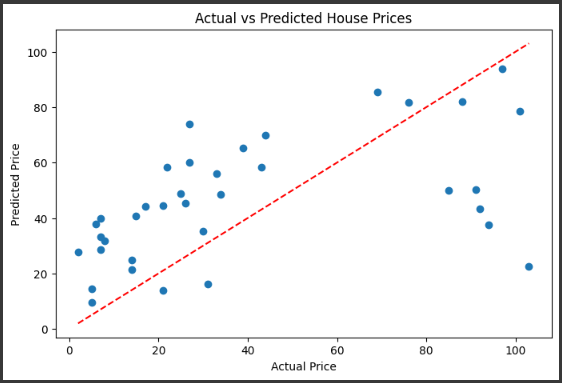
\includegraphics[width=0.8\textwidth]{figures/Screenshot_41.png}
\caption{Actual vs Predicted House Prices}
\label{fig:scatter_plot}
\end{figure}

As observed in Figure~\ref{fig:scatter_plot}, most points are closely aligned along the reference line, although some deviations are present. This behavior suggests that while the model performs well overall, there are a few instances where the predicted prices deviate from the actual values, particularly in extreme price ranges.

Overall, the experimental results validate the proposed approach, and provide a solid baseline for future improvements, such as incorporating multi-modal feature extraction and attention-based fusion mechanisms to further enhance accuracy.

\chapter{Conclusion}

In this project, we explored the problem of house price prediction at a subregion level using machine learning techniques. By leveraging a fully connected neural network architecture, we built a model capable of learning complex patterns and relationships within real estate datasets. Unlike traditional regression methods, our approach captured non-linear dependencies and provided more accurate predictive outputs.

The model was trained and evaluated on datasets from two major cities, New York City and Beijing. The achieved RMSE values of 21.43 and 60.19 respectively demonstrate that even a simplified neural network can outperform basic machine learning models in capturing property valuation trends. The training and validation curves indicated that the model generalized well without significant overfitting, while scatter plot analysis confirmed a strong correlation between predicted and actual house prices.

However, the project also revealed certain limitations. Due to the simplicity of the network architecture, extreme variations in property prices (outliers) were not always predicted accurately. Additionally, external economic factors, demographic shifts, and geographic influences were not fully integrated into the current model, limiting its overall predictive capability.

Looking forward, several improvements can be made to enhance the system:
\begin{itemize}
    \item Implementing multi-branch feature extraction to separately handle short-term and long-term features.
    \item Introducing Gated Co-Attention mechanisms to dynamically focus on the most relevant features during prediction.
    \item Utilizing future expectation modeling through techniques like Kalman Filters to capture upcoming market trends.
    \item Expanding the dataset by integrating socio-economic indicators, geographic data, and neighborhood statistics for more comprehensive modeling.
\end{itemize}

Overall, the work accomplished in this project lays a strong foundation for advanced predictive modeling in the real estate sector. It opens opportunities to develop intelligent, data-driven decision-making tools that can benefit buyers, sellers, investors, and urban planners by providing accurate and timely property valuations.

\chapter*{Contribution of Each Member}

The following outlines the contributions made by each team member towards the successful completion of this project:

\begin{itemize}
    \item \textbf{ MD AMRAN HAQUE (ID: 221-15-5662)} - Worked on literature review, theoretical analysis, and helped design the initial model architecture makeing, Overleaf file and Overall Lead
    \item \textbf{MD TAHSINUL HOQUE (ID: 221-15-4661)} - Focused on dataset preprocessing, model training, and performance evaluation.Presention Slide make , paper analyis .
  
\end{itemize}

we are try to  collaboratively contributed towards discussions, report writing, proofreading, and final presentation preparation.




   
   
   

\clearpage

\end{document}
